
\section{Trading Strategies}
\label{chap:trading-strategies}

In the context of automated trading, systematic trading strategies play a central role.
They enable decisions to be made based on clearly defined rules or mathematical models, rather than on subjective assessments or human intuition.

A trading strategy defines a methodical approach by which financial instruments are bought or sold to achieve a specific goal.
Typically, this is to maximize profit while limiting risk.
Such strategies are often based on indicators from technical analysis or fundamental market information \cite{investopia-trading-strategy}.

Essential components of a strategy are signal generation (entry/exit criteria), risk management (e.g., stop-loss, position sizes), and performance evaluation based on metrics such as cumulative profit, or maximum drawdown.
The development process of a successful strategy typically comprises several phases, ranging from idea generation and backtesting to optimization and validation on previously unseen market data \cite{investopia-trading-strategy-components}.

Similar to deep learning hyperparameters, trading strategies also involve adjustable parameters that mus be defined before execution.
In this work, these parameters are defined in a range, consisting of a minimal value, a maximum value, and a step size.
This setup allows for a structured and repeatable parameter search, enabling the systematic exploration of different strategy configurations.

This chapter provides an overview of the trading strategies compared in this paper.
Both the models trained in \autoref{chap:dl-models} and classic trading strategies are presented.
An overview of the metrics used to compare the trading strategies is also provided.
The presented strategies also have their parameters defined, which will be tested later.
It should be noted that each strategy also contains a parameter that defines whether positions are opened with a fixed stop level or a trailing stop.
Since this parameter is included in all strategies, it is not listed every time.

\subsection{AI Trading Strategies}
\label{chap:ai-strategies}

AI trading strategies treat the model outputs differently depending on whether the underlying model is based on regression or classification.
This variation arises from the fundamental nature of the models themselves and influences how their predictions are interpreted.

\subsubsection{Regression AI Strategy}
\label{chap:regression-ai-stategy}

As described in \autoref{chap:regression-models-evaluation}, the trained regression models are not suitable for developing a trading strategy.
Nevertheless, this chapter describes a trading strategy that could be implemented using a predicted series of logarithmic returns.
However, it is not evaluated or tested.

From the predicted series of logarithmic returns, the expected price in $t$ minutes can be calculated by the formula mentioned in \autoref{chap:log-returns}.

Based on the predicted price, the stop-loss and take-profit can be determined identically to the loss-function of the regression models (\autoref{chap:regression-loss}).
This creates an entry signal with fixed stop-loss and take-profit level.

However, since it is possible that the price could exceed the stop level or the take-profit level might not be reached, additional parameters are introduced into the strategy that shift the two levels by a specific number of points.
A third parameter is also introduced, which specifies a fixed distance to the stop-loss if no stop-loss has been predicted.
This can happen, for example, if the initial prediction is positive and the price in the prediction does not fall below the current price.

\begin{table}[H]
    \centering
    \begin{tabular}{L{4cm}ccc}
        \toprule
        \textbf{Parameter Name} & Min Value & Max Value & Step Size
        \\
        \midrule
        \textbf{Take-Profit Delta}             & -20.0 & 20.0 & 2.0  \\
        \textbf{Stop-Loss Delta}               & -20.0 & 20.0 & 2.0  \\
        \textbf{Stop-Loss not Predicted Delta} & 1.0   & 20.0 & 20.0 \\
        \bottomrule
    \end{tabular}
    \caption{AI Regression Model Strategy Parameters}
    \label{tbl:regression-strategy-parameters}
\end{table}

\subsubsection{Classification AI Strategy}

As described in \autoref{chap:classification-models} the classification models predict a probability for an action, which can be either buy, sell or do nothing.
The strategy evaluates these predicted probabilities and takes action only when certain conditions are met.
Specifically, a long or short entry signal is generated only if the corresponding predicted probability exceeds a predefined minimum threshold.
This ensures that trades are only placed when the model is sufficiently confident in its prediction.

If neither the buy nor the sell probability reached the minimum threshold, the strategy chooses to do nothing or stay out of the market.
This mechanism helps to filter out uncertain or low-confidence predictions, reducing the likelihood of unnecessary or potential unprofitable trades.

In addition to the action selection logic, the strategy also relies on predefined stop-loss and take-profit levels to manage risk and lock profits.


\begin{table}[H]
    \centering
    \begin{tabular}{L{4cm}ccc}
        \toprule
        \textbf{Parameter Name} & Min Value & Max Value & Step Size
        \\
        \midrule
        \textbf{Take-Profit Distance}       & 5.0 & 100.0 & 5.0 \\
        \textbf{Stop-Loss Distance}         & 5.0 & 100.0 & 5.0 \\
        \textbf{Min. Probability for Entry} & 0.3 & 0.9   & 0.1 \\
        \bottomrule
    \end{tabular}
    \caption{AI Classification Model Strategy Parameters}
    \label{tbl:classification-strategy-parameters}
\end{table}

\subsection{Classic Trading Strategies}

Technical analysis (TA) is based on the assumption that market movements do not develop randomly, but follow certain patterns that have repeated themselves in the past.
In contrast to fundamental analysis, which deals with the intrinsic value of a financial instrument, technical analysis focuses exclusively on past price and volume movements to draw conclusions about future price developments.

Technical analysis focuses on visual and computational methods for identifying trend, support and resistence levels, and reversal points.
These analysis are used to develop specific trading strategies that specifically respond to specific market behaviours.
These strategies are often rule-based and can be implemented both manually and algorithmically \cite{ta-basics}.
Therefore, technical analysis strategies are more likely suitable for algorithmic trading.

This chapter describes three widely used technical analysis trading strategies.
The strategies introduced are not the only classic strategies tested.
They are the three that performed best in the tests.
The other tested strategies are also briefly listed in \autoref{chap:other-strategy-results}.
However, some of them have been slightly modified in this work compared to the most widely used ones.

\subsubsection{Dual Simple Moving Average Strategy}
\label{chap:sma2}

A common trading strategy is the simple moving average crossover strategy.
It consists of two SMA with different periods.
If the short-term SMA crosses the long-term SMA above, a long position is opened.
Otherwise, if the short-term SMA crosses the long-term SMA below, a short position is opened \cite{sma-strategy-basics}.
\autoref{fig:sma-example} shows exemplary two moving averages for a synthetic price, with blue arrows marking buy entry signals and red arrows marking sell entry signals.

\begin{figure}[H]
    \centering
    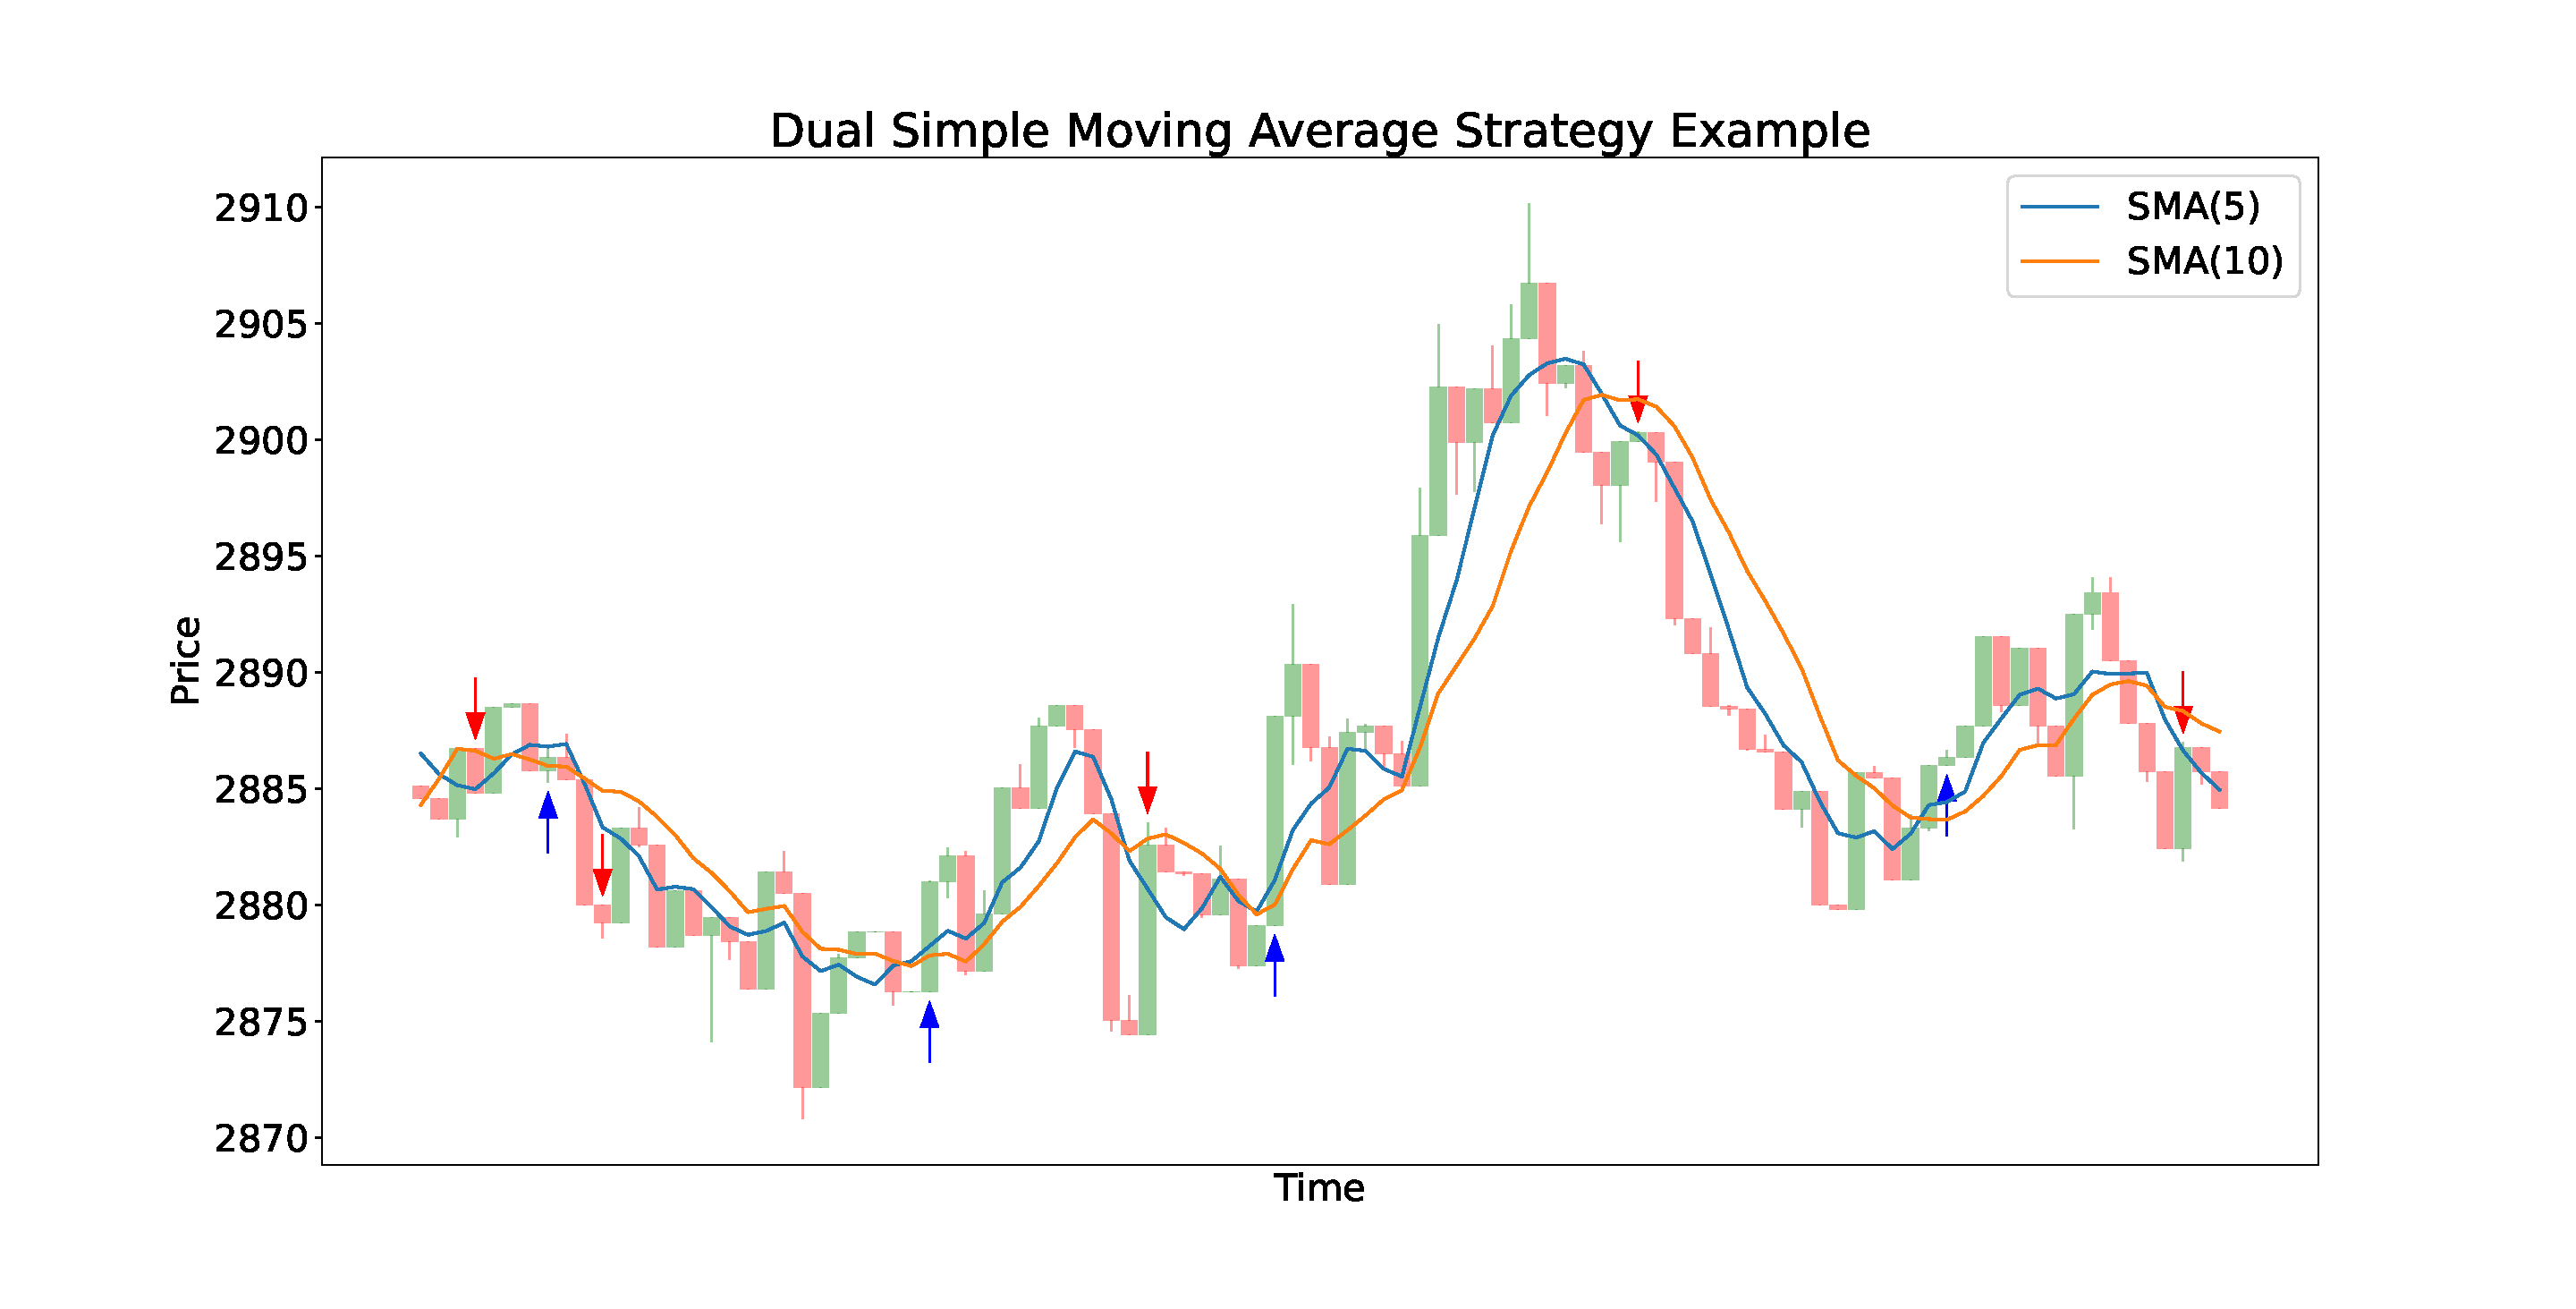
\includegraphics[width=\textwidth]{images/trading-strategies/sma-example}
    \caption{Dual Simple Moving Average Strategy Example}
    \label{fig:sma-example}
\end{figure}

\noindent
This strategy is straightforward to understand and implement and can help to identify possible trend changes which generate entry and exit signals.
One of the greatest disadvantages is that the SMA is a lagging indicator and in quickly changing market conditions, the signals can be delayed.
Especially in sideways market regimes, the SMAs can cross often, which can lead to false signals \cite{sma-advantage-disadvantage}.
Here, the market regime recognition plays an important role.
Through this, the strategy can be disabled in sideways regimes and enabled if the market has a clear trend.

Often the criteria for stop-loss and take-profit levels are percentage and risk-reward ratio based, which means that the stop-loss has a fixed distance, e.g., 2\% and the take-profit is e.g. double the distance of the stop-loss distance (relative to the current price) \cite{sma-sl-tp}.
To achieve a more adaptive stop-loss and take-profit level determination, a self-developed mechanism called swing detection was added.

This detection method identifies swings in price movements and differentiates between swing high and swing low points.
A swing high point at time $t$ is a point where the closing price is greater than all closing prices in the intervall $[t-N; t+N]$.
Similarly, a swing low point is a point where the closing price is lower than all closing prices in the same intervall.
This allows detecting simple support and resistence zones, on which the stop-loss can be set.
Therefore, the strategy adapts to the current market behaviour.

%\autoref{fig:swing-high-low} shows syntetic price movements where at time $t=0$ swing highs are detected.

%TODO: Chart für swing highs und lows

The strategy has six parameters, consisting of the long-term and short-term SMA period, the order $N$ of the swing detection, which determines how significant the swing has to be, the maximum age of the last swing point, as well as a delta for the stop-loss and take-profit levels (identically to those in \autoref{chap:regression-ai-stategy}).
All parameter combinations where the short-term SMA period is greater than the long-term SMA period, have been filtered out and are not tested.

\begin{table}[H]
    \centering
    \begin{tabular}{L{4cm}ccc}
        \toprule
        \textbf{Parameter Name} & Min Value & Max Value & Step Size
        \\
        \midrule
        \textbf{Short-Term SMA Period} & 1   & 10    & 1    \\
        \textbf{Long-Term SMA Period}  & 2   & 20    & 1    \\
        \textbf{Swing Order $N$}       & 1   & 10    & 1    \\
        \textbf{Take-Profit Delta}     & 0.0 & 200.0 & 10.0 \\
        \textbf{Stop-Loss Delta}       & 0.0 & 100.0 & 10.0 \\
        \bottomrule
    \end{tabular}
    \caption{Dual Simple Moving Average Strategy Parameters}
    \label{tbl:sma-strategy-parameters}
\end{table}

\subsubsection{Triple Exponential Moving Average Strategy}

This strategy consists of three exponential moving averages (EMA) with different periods.
The shortest EMA identifies short-term trends, while the medium EMA identifies medium-term trends, and the long EMA identifies long-term trend.

The common application of the triple exponential moving average strategy generates a buy signal if the short-term EMA crosses above the medium-term EMA.
Additionally, the medium-term EMA must already be above the long-term EMA to validate the buy signal.
For sell signals, the short-term EMA must cross below the medium-term EMA and the medium-term EMA has to be bellow the long-term EMA \cite{ema3-basics}.

Therefore, the long-term EMA acts as a trend filter to reduce false positives mentioned in \autoref{chap:sma2}.
In this work, the long-term EMA is also used as a trend filter but not by its position relative to two other EMA's.
During the backtesting of the classic variant, it was noticed that many false entry signals were still generated, especially in sideways markets.
Therefore, the trend was filtered using a minimal slope of the long-term EMA.
The slope of the EMA is calculated by the slope of the regression line which is defined by the current EMA value (at time $t$) and the EMA value $i$ minutes in the past.

\[
    Slope = \frac{EMA_t - EMA_{t-i}}{i}
\]

\noindent
If the slope is greater than a predefined threshold, only long positions can be opened.
On the other hand, if the slope is less than the negated threshold, only short positions can be opened.
Otherwise, the strategy cannot open any new positions.

\autoref{fig:ema-example} shows the same synthetic price as in \autoref{fig:sma-example}.
Additionally, a third EMA with period 20 is added, which is used to calculate the slope.
The red-filled areas indicate zones where no positions can be opened.
So the entry signals in these areas are ignored.
In the green-filled areas, the entry signals are executed.

\begin{figure}[H]
    \centering
    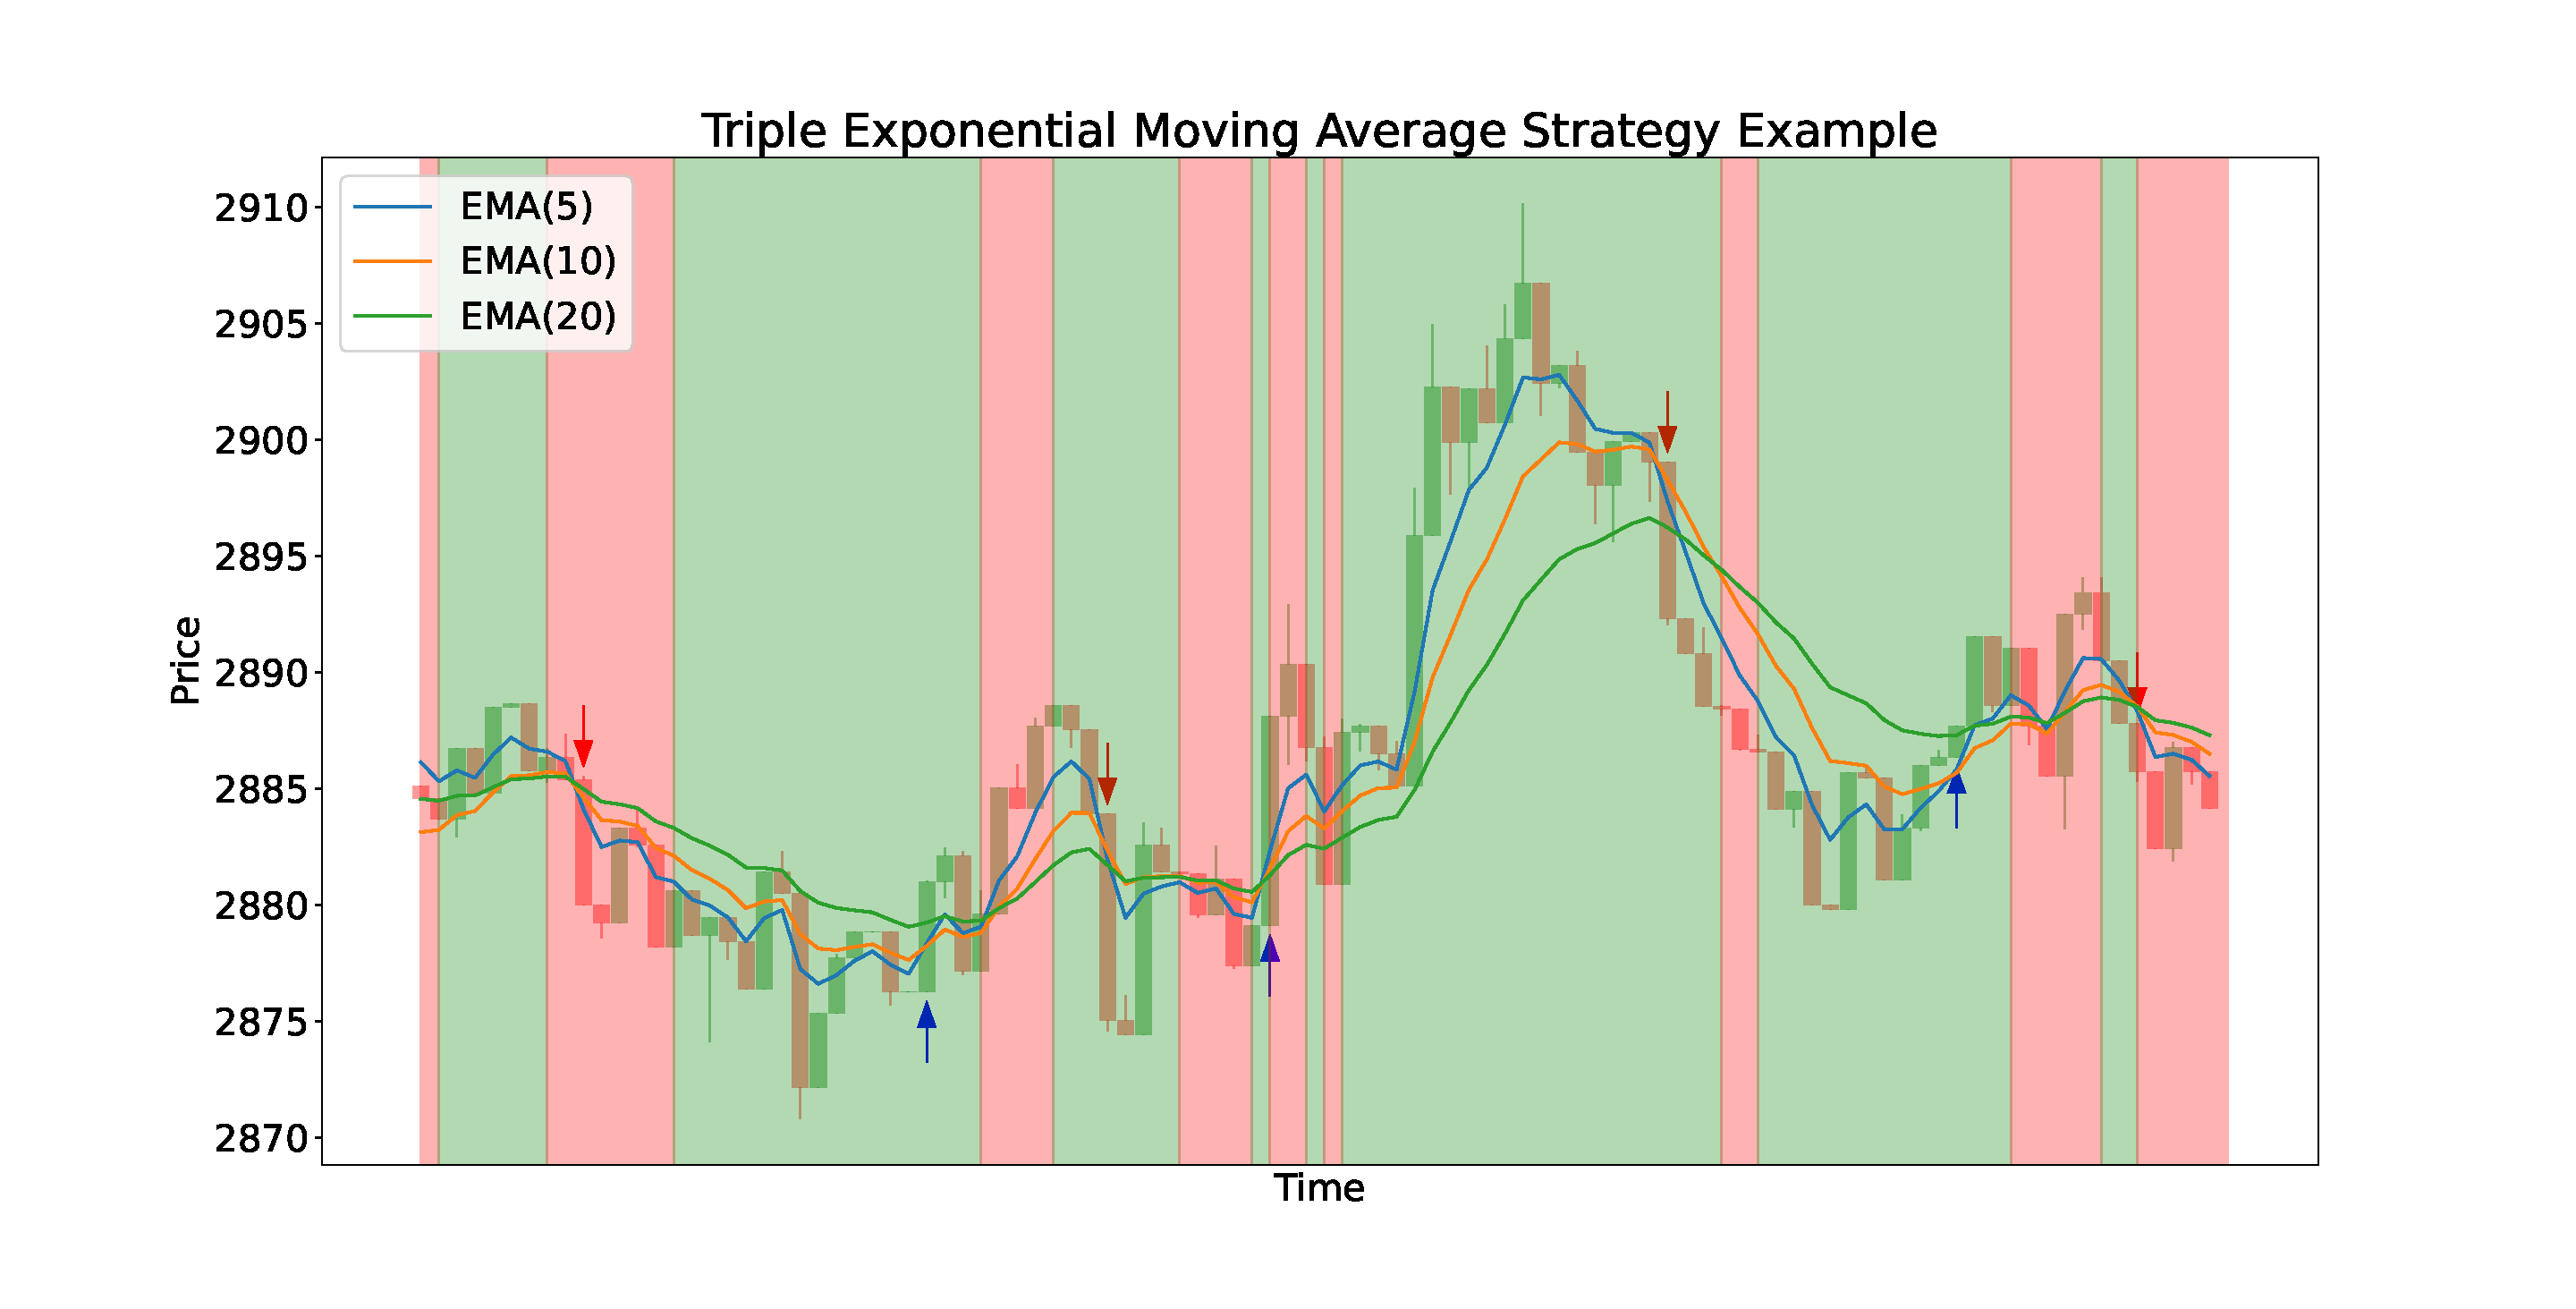
\includegraphics[width=\textwidth]{images/trading-strategies/ema-example}
    \caption{Triple Exponential Moving Average Strategy Example}
    \label{fig:ema-example}
\end{figure}

\noindent
In this strategy, the stop-loss and take-profit distance have been added as fixed parameters, which are also permuted.
All parameter combinations, where the short-term EMA period is greater than the medium-term EMA period, or the medium-term EMA period is greater than the long-term EMA period, are filtered out.

\begin{table}[H]
    \centering
    \begin{tabular}{L{4cm}ccc}
        \toprule
        \textbf{Parameter Name} & Min Value & Max Value & Step Size
        \\
        \midrule
        \textbf{Short-Term EMA Period}       & 3   & 10  & 2   \\
        \textbf{Medium-Term EMA Period}      & 5   & 30  & 3   \\
        \textbf{Long-Term EMA Period}        & 10  & 50  & 5   \\
        \textbf{Minimum EMA Slope}           & 0.2 & 1.2 & 0.2 \\
        \textbf{EMA Slope Window Length $i$} & 10  & 40  & 10  \\
        \textbf{Stop-Loss Distance}          & 10  & 100 & 10  \\
        \textbf{Take-Profit Distance}        & 10  & 150 & 10  \\
        \bottomrule
    \end{tabular}
    \caption{Triple Exponential Moving Average Strategy Parameters}
    \label{tbl:ema-strategy-parameters}
\end{table}

\subsubsection{Bollinger Bands Strategy}

The Bollinger Bands strategy is a mean reversion strategy, designed to exploit short-term price fluctuations.
This strategy assumes that after approaching or breaking through the outer bands, the price reverts to the central line (the moving average).
A buy entry signal is generated if a candle opens below the lower Bollinger Band and closes above the lower Bollinger Band.
This indicates a price reversal from an oversold condition.
On the other hand, a sell entry signal is generated if the candle opens above the upper Bollinger Band and closes below the upper Bollinger Band \cite{bb-basics}.

\autoref{fig:bb-example} shows the synthetic price, identically to \autoref{fig:sma-example} and \autoref{fig:ema-example}.
The blue-filled area shows the Bollinger Band, with the central line.

\begin{figure}[H]
    \centering
    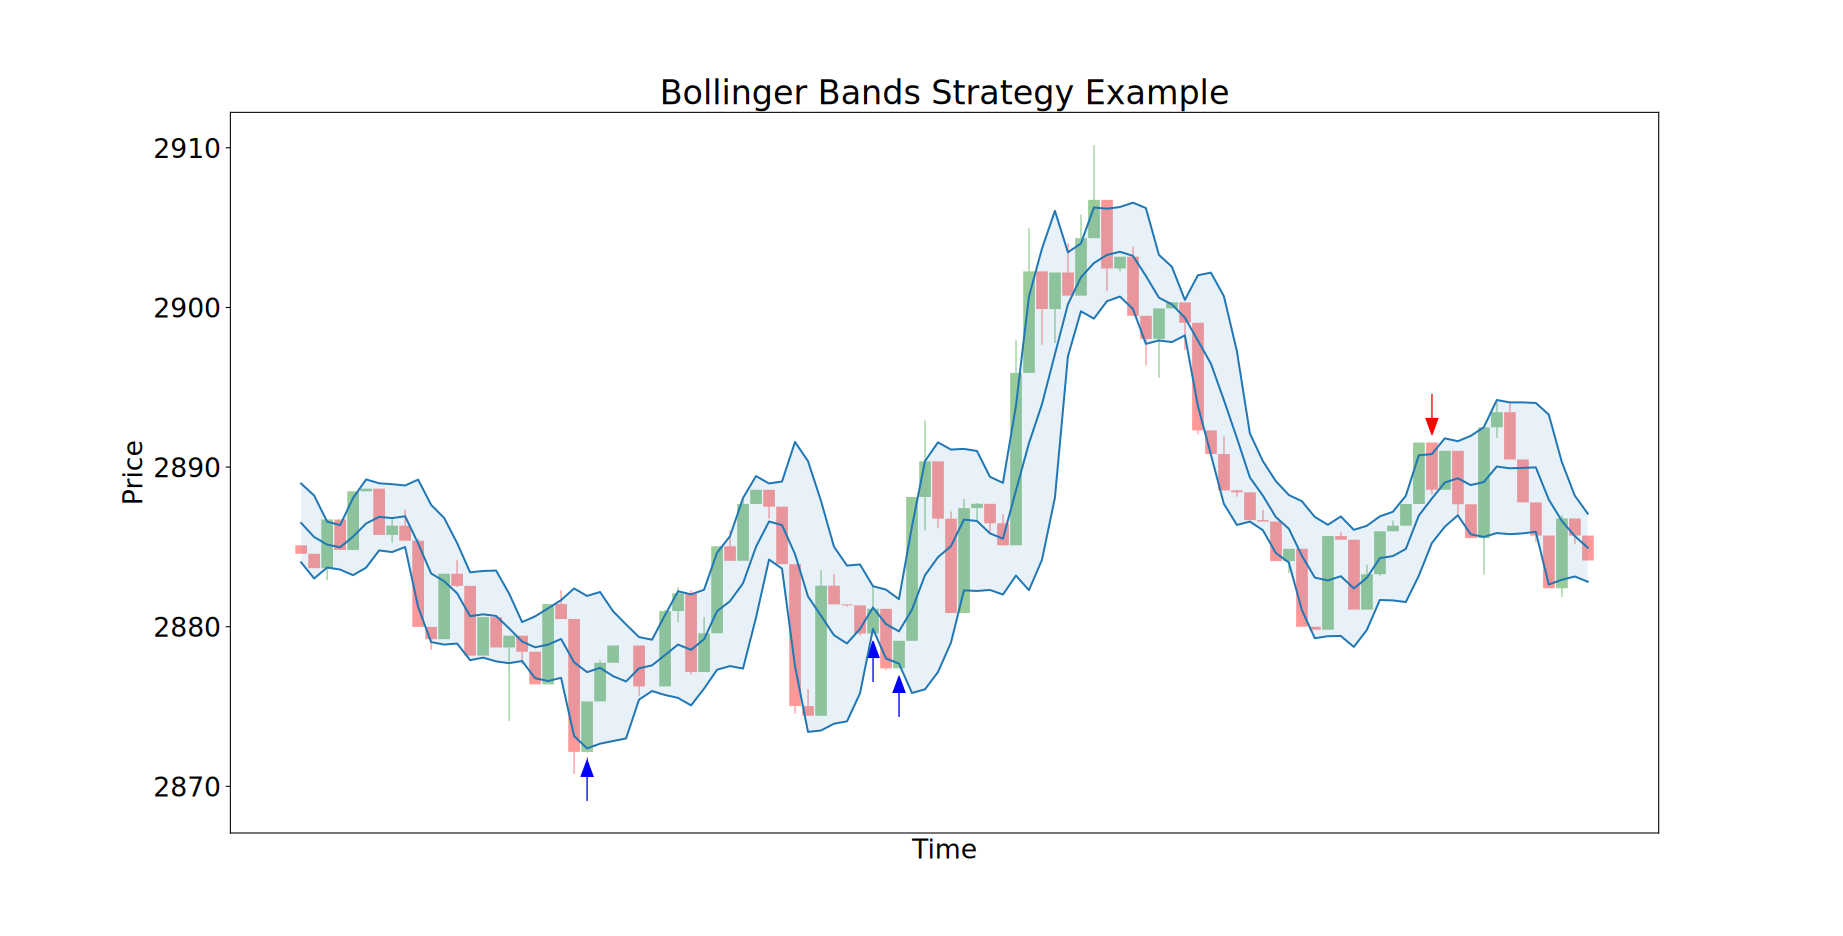
\includegraphics[width=\textwidth]{images/trading-strategies/bb-example}
    \caption{Bollinger Bands Strategy Example}
    \label{fig:bb-example}
\end{figure}

\noindent
The stop-loss level is set in a predefined distance relative to the current price.
The take-profit level is set at the level of the central line , with a certain delta being added (for buy signals) or subtracted (for sell signals) to the value of the middle line.

\begin{table}[H]
    \centering
    \begin{tabular}{L{4cm}ccc}
        \toprule
        \textbf{Parameter Name} & Min Value & Max Value & Step Size
        \\
        \midrule
        \textbf{Bollinger Band Period}      & 10   & 25    & 1    \\
        \textbf{No. of Standard Deviations} & 1.5  & 3.0   & 0.5  \\
        \textbf{Stop-Loss Distance}         & 10.0 & 100.0 & 20.0 \\
        \textbf{Take-Profit Delta}          & -5.0 & 20.0  & 2.0  \\
        \bottomrule
    \end{tabular}
    \caption{Bollinger Band Strategy Parameters}
    \label{tbl:bb-strategy-parameters}
\end{table}
